\documentclass[12pt,a4paper]{article}
\usepackage{amsmath,amssymb,amsfonts}
\usepackage{graphicx}
\usepackage{tikz}
\usepackage{float}
\usepackage{hyperref}
\usepackage{xcolor}
\usepackage{tcolorbox}
\usepackage{enumitem}
\usepackage{calc}

\usetikzlibrary{arrows,shapes,positioning,shadows,trees,decorations.pathreplacing,calc}

\hypersetup{
    colorlinks=true,
    linkcolor=blue,
    filecolor=magenta,
    urlcolor=cyan,
}

\title{2. Reinforcement Learning: From Bandits to Full RL}


\begin{document}

\maketitle
\tableofcontents
\newpage

\section{Introduction}
This document covers the transition from the multi-armed bandit problem to full reinforcement learning, exploring how the introduction of states transforms the problem and solution approaches. We follow the notation and framework established in Sutton and Barto's Reinforcement Learning book.

\section{Associativity: Reward Dependency on States and Actions}
\subsection{From Simple Bandits to State-Dependent Rewards}

In the multi-armed bandit problem, rewards depend only on the selected action:
\begin{equation}
p(r_t|a_t)
\end{equation}

\begin{tcolorbox}[title=Notation Overview]
\begin{itemize}
    \item $p(r_t|a_t)$ - The probability distribution of reward $r_t$ given action $a_t$
    \item $r_t$ - The reward received at time step $t$
    \item $a_t$ - The action taken at time step $t$
\end{itemize}
\end{tcolorbox}

Associativity introduces the concept of state, where rewards now depend on both the current state and the action taken:
\begin{equation}
p(r_t|s_t, a_t)
\end{equation}

\begin{tcolorbox}[title=Notation Overview]
\begin{itemize}
    \item $p(r_t|s_t, a_t)$ - The probability distribution of reward $r_t$ given state $s_t$ and action $a_t$
    \item $r_t$ - The reward received at time step $t$
    \item $s_t$ - The state at time step $t$
    \item $a_t$ - The action taken at time step $t$
\end{itemize}
\end{tcolorbox}

In reinforcement learning with associativity, the agent recognizes that the environment is not stationary but exists in different states. The reward received for a particular action depends not only on which action was chosen but also on the environmental state in which it was chosen.

\subsection{The Agent-Environment Interface}

The standard agent-environment interface in reinforcement learning extends the bandit formulation to include states:

\begin{figure}[H]
\centering
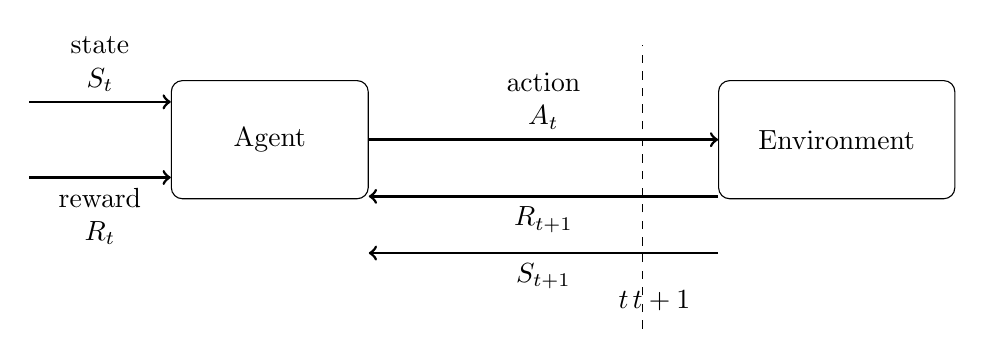
\begin{tikzpicture}[scale=1.2]
    % Boxes for Agent and Environment
    \node[draw, rounded corners, minimum width=2.5cm, minimum height=1.5cm] (agent) at (0,0) {Agent};
    \node[draw, rounded corners, minimum width=3cm, minimum height=1.5cm] (env) at (6,0) {Environment};
    
    % Action arrow from Agent to Environment
    \draw[->, line width=1pt] (agent.east) -- node[above, align=center] {action\\$A_t$} (env.west);
    
    % Reward and State arrows from Environment to Agent
    \draw[->, line width=1pt] (env.west |- 0,-0.6) -- node[below, align=center] {$R_{t+1}$} (agent.east |- 0,-0.6);
    \draw[->, line width=1pt] (env.west |- 0,-1.2) -- node[below, align=center] {$S_{t+1}$} (agent.east |- 0,-1.2);
    
    % State and Reward arrows to Agent (left side)
    \draw[->, line width=1pt] ($(agent.west) + (-1.5,0.4)$) -- node[above, align=center] {state\\$S_t$} ($(agent.west) + (0,0.4)$);
    \draw[->, line width=1pt] ($(agent.west) + (-1.5,-0.4)$) -- node[below, align=center] {reward\\$R_t$} ($(agent.west) + (0,-0.4)$);
    
    % Dotted line separating time steps
    \draw[dashed] ($(env.west) + (-0.8,-2)$) -- ($(env.west) + (-0.8,1)$);
    
    % Labels for t and t+1
    \node at ($(env.west) + (-1.0,-1.7)$) {$t$};
    \node at ($(env.west) + (-0.6,-1.7)$) {$t+1$};
\end{tikzpicture}
\caption{The agent-environment interaction in reinforcement learning (Sutton \& Barto)}
\end{figure}

At each time step $t$:
\begin{itemize}
    \item The agent observes the current state $S_t \in \mathcal{S}$
    \item Based on this state, the agent selects an action $A_t \in \mathcal{A}(S_t)$
    \item The environment responds with a reward $R_{t+1} \in \mathcal{R}$ and a new state $S_{t+1}$
    \item The agent then selects a new action based on the new state, and the process continues
\end{itemize}

This creates a sequence of states, actions, and rewards:
\begin{equation}
S_0, A_0, R_1, S_1, A_1, R_2, S_2, A_2, R_3, \ldots
\end{equation}

\begin{tcolorbox}[title=Notation Overview]
\begin{itemize}
    \item $S_t$ - The state at time step $t$
    \item $A_t$ - The action taken at time step $t$
    \item $R_{t+1}$ - The reward received after taking action $A_t$ in state $S_t$
    \item $\mathcal{S}$ - The set of all possible states
    \item $\mathcal{A}(S_t)$ - The set of actions available in state $S_t$
    \item $\mathcal{R}$ - The set of possible rewards
\end{itemize}
\end{tcolorbox}

\subsection{The Markov Property}

A key concept in reinforcement learning is the Markov property, which states that the future is independent of the past given the present. Formally, an environment has the Markov property if:

\begin{equation}
P(S_{t+1}=s', R_{t+1}=r | S_t, A_t, R_t, S_{t-1}, A_{t-1}, \ldots, R_1, S_0, A_0) = P(S_{t+1}=s', R_{t+1}=r | S_t, A_t)
\end{equation}

\begin{tcolorbox}[title=Notation Overview]
\begin{itemize}
    \item $P(S_{t+1}=s', R_{t+1}=r | S_t, A_t, \ldots)$ - The probability of transitioning to state $s'$ and receiving reward $r$ given the entire history
    \item $P(S_{t+1}=s', R_{t+1}=r | S_t, A_t)$ - The probability of transitioning to state $s'$ and receiving reward $r$ given only the current state and action
    \item $S_t$ - The state at time step $t$
    \item $A_t$ - The action taken at time step $t$
    \item $R_t$ - The reward received at time step $t$
\end{itemize}
\end{tcolorbox}

The Markov property is crucial because it allows us to make decisions based solely on the current state without needing to remember the entire history of states and actions. This simplifies the problem significantly while still capturing the essential dynamics of many real-world situations.

\section{Extension to Contextual Bandits}
\subsection{Definition and Properties}

Contextual bandits represent an intermediate step between multi-armed bandits and full reinforcement learning. In this setting:

\begin{itemize}
    \item The environment presents a state (or context) $S_t$ to the agent
    \item The agent chooses an action $A_t$ based on the state
    \item The environment provides a reward $R_{t+1}$ that depends on both $S_t$ and $A_t$
    \item The next state $S_{t+1}$ is \textbf{not influenced} by the previous action $A_t$
\end{itemize}

The key distinguishing feature of contextual bandits is that while rewards depend on states, actions do not influence future states. The state transitions are independent of the agent's actions:

\begin{equation}
p(s_{t+1}|s_t, a_t) = p(s_{t+1}|s_t)
\end{equation}

\begin{tcolorbox}[title=Notation Overview]
\begin{itemize}
    \item $p(s_{t+1}|s_t, a_t)$ - The probability of transitioning to state $s_{t+1}$ given the current state $s_t$ and action $a_t$
    \item $p(s_{t+1}|s_t)$ - The probability of transitioning to state $s_{t+1}$ given only the current state $s_t$, independent of the action taken
    \item $s_t$ - The state at time step $t$
    \item $a_t$ - The action taken at time step $t$
    \item $s_{t+1}$ - The next state at time step $t+1$
\end{itemize}
\end{tcolorbox}

\subsection{Applications of Contextual Bandits}

Contextual bandits are particularly useful in scenarios where:

\begin{itemize}
    \item The state/context changes independently of the agent's actions
    \item Decisions only affect immediate rewards but not future states
    \item The agent needs to adapt to changing contexts
\end{itemize}

Some practical applications include:

\begin{itemize}
    \item News article recommendation: The user's interests (state) change over time independently of which articles are recommended, but the reward (click-through rate) depends on both the user's interests and the selected article.
    
    \item Dynamic pricing: Market conditions (state) change due to external factors, while the price decision (action) affects immediate revenue but not future market conditions.
    
    \item Clinical trials with rotating patients: Each patient represents a new state, and the treatment decision affects the outcome for that patient but not the characteristics of future patients.
\end{itemize}

\subsection{Action-Value Function for Contextual Bandits}

In contextual bandits, the action-value function is defined as the expected immediate reward when taking action $a$ in state $s$:

\begin{equation}
Q(s,a) = \mathbb{E}[R_{t+1}|S_t = s, A_t = a]
\end{equation}

\begin{tcolorbox}[title=Notation Overview]
\begin{itemize}
    \item $Q(s,a)$ - The action-value function, representing the expected reward for taking action $a$ in state $s$
    \item $\mathbb{E}[\cdot]$ - The expected value
    \item $R_{t+1}$ - The reward received at time step $t+1$
    \item $S_t$ - The state at time step $t$
    \item $A_t$ - The action taken at time step $t$
\end{itemize}
\end{tcolorbox}

This differs from the action-value function in full reinforcement learning, which includes future rewards.

\subsection{Estimating Action Values in Contextual Bandits}

The action-value function in contextual bandits can be estimated from experience:

\begin{equation}
Q_t(s,a) = \frac{1}{n_t(s,a)} \sum_{i=1}^{t} r_i \cdot \mathbb{I}(s_i = s, a_i = a)
\end{equation}

\begin{tcolorbox}[title=Notation Overview]
\begin{itemize}
    \item $Q_t(s,a)$ - The estimated action-value after $t$ steps
    \item $n_t(s,a)$ - The number of times action $a$ has been selected in state $s$ up to time $t$
    \item $r_i$ - The reward received at step $i$
    \item $\mathbb{I}(s_i = s, a_i = a)$ - An indicator function that equals 1 if $s_i = s$ and $a_i = a$, and 0 otherwise
    \item $s_i$ - The state at time step $i$
    \item $a_i$ - The action taken at time step $i$
\end{itemize}
\end{tcolorbox}

An incremental update rule for the action values can also be derived:

\begin{equation}
Q_{t+1}(s_t,a_t) = Q_t(s_t,a_t) + \alpha [r_{t+1} - Q_t(s_t,a_t)]
\end{equation}

\begin{tcolorbox}[title=Notation Overview]
\begin{itemize}
    \item $Q_{t+1}(s_t,a_t)$ - The updated estimate of the action-value
    \item $Q_t(s_t,a_t)$ - The current estimate of the action-value
    \item $\alpha$ - The step-size parameter (learning rate), $0 < \alpha \leq 1$
    \item $r_{t+1}$ - The observed reward
    \item $s_t$ - The state at time step $t$
    \item $a_t$ - The action taken at time step $t$
\end{itemize}
\end{tcolorbox}

\subsection{Policy in Contextual Bandits}

A policy $\pi$ in contextual bandits maps states to probabilities of selecting each possible action:

\begin{equation}
\pi(a|s) = P(A_t = a | S_t = s)
\end{equation}

\begin{tcolorbox}[title=Notation Overview]
\begin{itemize}
    \item $\pi(a|s)$ - The probability of selecting action $a$ in state $s$ under policy $\pi$
    \item $P(A_t = a | S_t = s)$ - The probability that the agent selects action $A_t = a$ when in state $S_t = s$
    \item $A_t$ - The action taken at time step $t$
    \item $S_t$ - The state at time step $t$
\end{itemize}
\end{tcolorbox}

Various policy types can be used in contextual bandits:

\begin{itemize}
    \item \textbf{Greedy Policy}: Always selects the action with the highest estimated value:
    \begin{equation}
    \pi(a|s) = 
    \begin{cases}
    1 & \text{if } a = \arg\max_{a'} Q(s,a') \\
    0 & \text{otherwise}
    \end{cases}
    \end{equation}
    
    \item \textbf{$\epsilon$-Greedy Policy}: Selects the best action most of the time, but occasionally explores:
    \begin{equation}
    \pi(a|s) = 
    \begin{cases}
    1 - \epsilon + \frac{\epsilon}{|\mathcal{A}(s)|} & \text{if } a = \arg\max_{a'} Q(s,a') \\
    \frac{\epsilon}{|\mathcal{A}(s)|} & \text{otherwise}
    \end{cases}
    \end{equation}
    
    \item \textbf{Softmax Policy}: Selects actions with probabilities proportional to their estimated values:
    \begin{equation}
    \pi(a|s) = \frac{e^{Q(s,a)/\tau}}{\sum_{a'} e^{Q(s,a')/\tau}}
    \end{equation}
    where $\tau$ is a temperature parameter controlling exploration.
\end{itemize}

\subsection{Example: Contextual Multi-Armed Bandit}

Consider a modified version of the multi-armed bandit problem where there are visible weather conditions (sunny, rainy, cloudy) that affect the rewards for each arm (e.g., different types of investments). The rewards for each arm depend on the weather, but today's action doesn't affect tomorrow's weather.

\begin{figure}[H]
\centering
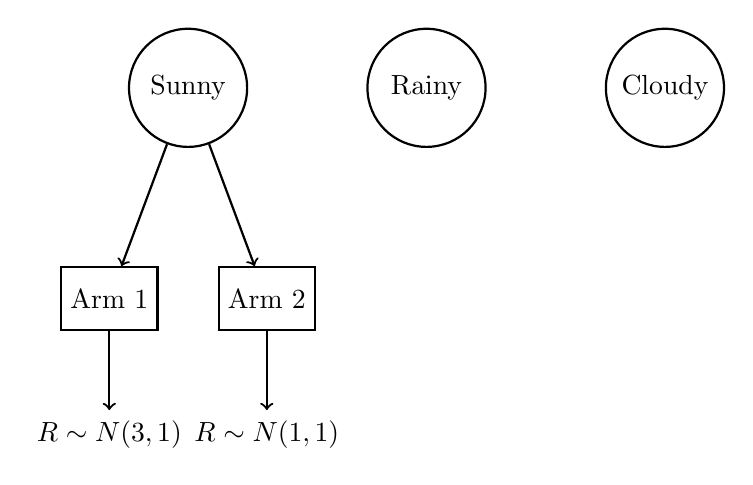
\begin{tikzpicture}[node distance=1.5cm, auto, thick]
    % Weather states
    \node[draw,circle,minimum size=1.5cm] (sunny) {Sunny};
    \node[draw,circle,minimum size=1.5cm, right=of sunny] (rainy) {Rainy};
    \node[draw,circle,minimum size=1.5cm, right=of rainy] (cloudy) {Cloudy};
    
    % Arms (actions)
    \node[draw,rectangle,minimum width=1.2cm,minimum height=0.8cm, below=of sunny, xshift=-1cm] (arm1) {Arm 1};
    \node[draw,rectangle,minimum width=1.2cm,minimum height=0.8cm, below=of sunny, xshift=1cm] (arm2) {Arm 2};
    
    % Rewards
    \node[below=of arm1, yshift=0.5cm] (reward1) {$R \sim N(3,1)$};
    \node[below=of arm2, yshift=0.5cm] (reward2) {$R \sim N(1,1)$};
    
    % Connect states to arms
    \draw[->] (sunny) -- (arm1);
    \draw[->] (sunny) -- (arm2);
    
    % Connect arms to rewards
    \draw[->] (arm1) -- (reward1);
    \draw[->] (arm2) -- (reward2);
    
    % Add more connections and details for other weather conditions
    % (simplified for clarity)
\end{tikzpicture}
\caption{A simplified contextual bandit example with weather states}
\end{figure}

The key insight is that while the agent's action choice depends on the observed state (weather), and the rewards depend on both state and action, the agent's actions do not influence which state occurs next.

\section{Full RL with State Transitions}
\subsection{The Critical Addition: Actions Affect Future States}

The defining characteristic of full reinforcement learning is that actions not only influence immediate rewards but also affect future states, and through them, future rewards:

\begin{equation}
p(s_{t+1}|s_t, a_t)
\end{equation}

\begin{tcolorbox}[title=Notation Overview]
\begin{itemize}
    \item $p(s_{t+1}|s_t, a_t)$ - The probability of transitioning to state $s_{t+1}$ given the current state $s_t$ and action $a_t$
    \item $s_t$ - The state at time step $t$
    \item $a_t$ - The action taken at time step $t$
    \item $s_{t+1}$ - The next state at time step $t+1$
\end{itemize}
\end{tcolorbox}

This introduces a critical complexity: actions have long-term consequences through their influence on future states. The agent must consider not just immediate rewards but also how actions shape future opportunities.

\subsection{Markov Decision Processes (MDPs)}

Full reinforcement learning problems are typically formalized as Markov Decision Processes (MDPs), which are defined by:

\begin{itemize}
    \item A set of states $\mathcal{S}$
    \item A set of actions $\mathcal{A}$
    \item A reward function $r(s, a) = \mathbb{E}[R_{t+1}|S_t = s, A_t = a]$
    \item A state transition probability function $p(s'|s, a) = P(S_{t+1} = s'|S_t = s, A_t = a)$
    \item A discount factor $\gamma \in [0, 1]$
\end{itemize}

The dynamics of an MDP are formally defined by:

\begin{equation}
p(s',r|s,a) = P(S_t = s', R_t = r|S_{t-1} = s, A_{t-1} = a)
\end{equation}

\begin{tcolorbox}[title=Notation Overview]
\begin{itemize}
    \item $p(s',r|s,a)$ - The probability of transitioning to state $s'$ and receiving reward $r$, given that the agent was in state $s$ and took action $a$
    \item $P(S_t = s', R_t = r|S_{t-1} = s, A_{t-1} = a)$ - The probability that the state at time $t$ is $s'$ and the reward is $r$, given that the state at time $t-1$ was $s$ and the action taken was $a$
    \item $S_t$ - The state at time step $t$
    \item $R_t$ - The reward received at time step $t$
    \item $A_t$ - The action taken at time step $t$
\end{itemize}
\end{tcolorbox}

From this joint probability function, we can derive other important quantities:

\begin{equation}
p(s'|s,a) = \sum_{r \in \mathcal{R}} p(s',r|s,a)
\end{equation}

\begin{equation}
r(s,a) = \mathbb{E}[R_t|S_{t-1}=s, A_{t-1}=a] = \sum_{r \in \mathcal{R}} r \sum_{s' \in \mathcal{S}} p(s',r|scla,a)
\end{equation}

\begin{equation}
r(s,a,s') = \mathbb{E}[R_t|S_{t-1}=s, A_{t-1}=a, S_t=s'] = \sum_{r \in \mathcal{R}} r \frac{p(s',r|s,a)}{p(s'|s,a)}
\end{equation}

\begin{tcolorbox}[title=Notation Overview]
\begin{itemize}
    \item $p(s'|s,a)$ - The probability of transitioning to state $s'$ given state $s$ and action $a$
    \item $r(s,a)$ - The expected reward when taking action $a$ in state $s$
    \item $r(s,a,s')$ - The expected reward when transitioning from state $s$ to state $s'$ via action $a$
    \item $\mathcal{R}$ - The set of possible rewards
    \item $\mathcal{S}$ - The set of possible states
\end{itemize}
\end{tcolorbox}

\subsection{Episodic vs. Continuing Tasks}

Reinforcement learning tasks can be categorized as either episodic or continuing:

\begin{itemize}
    \item \textbf{Episodic Tasks}: These have a clear endpoint or terminal state. For example, a game of chess ends with either a win, loss, or draw. The sequence of states, actions, and rewards from the start to the terminal state is called an episode.
    
    \item \textbf{Continuing Tasks}: These go on indefinitely without a natural endpoint. For example, an ongoing process control system or a stock trading agent that operates continuously.
\end{itemize}

\subsection{The Return and Value Functions in Full RL}

In full RL, the objective is to maximize the expected return, which is the cumulative discounted reward:

\begin{equation}
G_t = R_{t+1} + \gamma R_{t+2} + \gamma^2 R_{t+3} + \ldots = \sum_{k=0}^{\infty} \gamma^k R_{t+k+1}
\end{equation}

\begin{tcolorbox}[title=Notation Overview]
\begin{itemize}
    \item $G_t$ - The return at time step $t$
    \item $R_{t+k}$ - The reward received $k$ steps after time $t$
    \item $\gamma$ - The discount factor, $0 \leq \gamma \leq 1$
\end{itemize}
\end{tcolorbox}

For episodic tasks with a clear terminal state, we can alternatively define the return as:

\begin{equation}
G_t = \sum_{k=0}^{T-t-1} \gamma^k R_{t+k+1}
\end{equation}

where $T$ is the final time step of the episode.

To unify the notation for both episodic and continuing tasks, we can use:

\begin{equation}
G_t = \sum_{k=t+1}^{T} \gamma^{k-t-1} R_k
\end{equation}

with the understanding that $T=\infty$ for continuing tasks, and $\gamma < 1$ for continuing tasks to ensure the sum is finite.

\subsection{State-Value and Action-Value Functions}

The state-value function represents the expected return when starting in state $s$ and following policy $\pi$:

\begin{equation}
v_{\pi}(s) = \mathbb{E}_{\pi}[G_t|S_t = s] = \mathbb{E}_{\pi}\left[\sum_{k=0}^{\infty} \gamma^k R_{t+k+1} \bigg| S_t = s\right]
\end{equation}

\begin{tcolorbox}[title=Notation Overview]
\begin{itemize}
    \item $v_{\pi}(s)$ - The state-value function for policy $\pi$
    \item $\mathbb{E}_{\pi}[\cdot]$ - The expected value when following policy $\pi$
    \item $G_t$ - The return at time step $t$
    \item $S_t$ - The state at time step $t$
    \item $R_{t+k+1}$ - The reward received $k+1$ steps after time $t$
    \item $\gamma$ - The discount factor, $0 \leq \gamma \leq 1$
\end{itemize}
\end{tcolorbox}

Similarly, the action-value function represents the expected return when starting in state $s$, taking action $a$, and thereafter following policy $\pi$:

\begin{equation}
q_{\pi}(s,a) = \mathbb{E}_{\pi}[G_t|S_t = s, A_t = a] = \mathbb{E}_{\pi}\left[\sum_{k=0}^{\infty} \gamma^k R_{t+k+1} \bigg| S_t = s, A_t = a\right]
\end{equation}

\begin{tcolorbox}[title=Notation Overview]
\begin{itemize}
    \item $q_{\pi}(s,a)$ - The action-value function for policy $\pi$
    \item $\mathbb{E}_{\pi}[\cdot]$ - The expected value when following policy $\pi$
    \item $G_t$ - The return at time step $t$
    \item $S_t$ - The state at time step $t$
    \item $A_t$ - The action taken at time step $t$
    \item $R_{t+k+1}$ - The reward received $k+1$ steps after time $t$
    \item $\gamma$ - The discount factor, $0 \leq \gamma \leq 1$
\end{itemize}
\end{tcolorbox}

\subsection{The Relationship Between State-Value and Action-Value Functions}

The state-value and action-value functions are related by:

\begin{equation}
v_{\pi}(s) = \sum_{a} \pi(a|s) q_{\pi}(s, a)
\end{equation}

This shows that the value of a state is the expected value of the actions that might be taken in that state, weighted by their probability under policy $\pi$.

Conversely, we can express the action-value in terms of the state-value:

\begin{equation}
q_{\pi}(s, a) = \sum_{s', r} p(s', r|s, a) [r + \gamma v_{\pi}(s')]
\end{equation}

This indicates that the value of taking action $a$ in state $s$ is the expected immediate reward plus the discounted value of the next state.

\subsection{The Bellman Equations}

The recursive relationship between value functions is captured by the Bellman equations. For the state-value function:

\begin{equation}
v_{\pi}(s) = \sum_{a} \pi(a|s) \sum_{s',r} p(s',r|s,a) [r + \gamma v_{\pi}(s')]
\end{equation}

\begin{tcolorbox}[title=Notation Overview]
\begin{itemize}
    \item $v_{\pi}(s)$ - The state-value function for policy $\pi$
    \item $\pi(a|s)$ - The probability of selecting action $a$ in state $s$ under policy $\pi$
    \item $p(s',r|s,a)$ - The probability of transitioning to state $s'$ and receiving reward $r$, given state $s$ and action $a$
    \item $r$ - The reward
    \item $\gamma$ - The discount factor, $0 \leq \gamma \leq 1$
\end{itemize}
\end{tcolorbox}

And for the action-value function:

\begin{equation}
q_{\pi}(s,a) = \sum_{s',r} p(s',r|s,a) \left[r + \gamma \sum_{a'} \pi(a'|s') q_{\pi}(s',a') \right]
\end{equation}

\begin{tcolorbox}[title=Notation Overview]
\begin{itemize}
    \item $q_{\pi}(s,a)$ - The action-value function for policy $\pi$
    \item $p(s',r|s,a)$ - The probability of transitioning to state $s'$ and receiving reward $r$, given state $s$ and action $a$
    \item $\pi(a'|s')$ - The probability of selecting action $a'$ in state $s'$ under policy $\pi$
    \item $r$ - The reward
    \item $\gamma$ - The discount factor, $0 \leq \gamma \leq 1$
\end{itemize}
\end{tcolorbox}

The Bellman equations express a fundamental property: the value of a state (or state-action pair) equals the expected immediate reward plus the discounted value of the next state (or states).

\subsection{Optimal Value Functions and Policies}

A policy $\pi$ is defined as better than or equal to a policy $\pi'$ if its expected return is greater than or equal to that of $\pi'$ for all states:

\begin{equation}
\pi \geq \pi' \iff v_{\pi}(s) \geq v_{\pi'}(s) \text{ for all } s \in \mathcal{S}
\end{equation}

There is always at least one policy that is better than or equal to all other policies, called an optimal policy, denoted $\pi_*$. All optimal policies share the same optimal state-value function, $v_*$:

\begin{equation}
v_*(s) = \max_{\pi} v_{\pi}(s) \text{ for all } s \in \mathcal{S}
\end{equation}

They also share the same optimal action-value function, $q_*$:

\begin{equation}
q_*(s,a) = \max_{\pi} q_{\pi}(s,a) \text{ for all } s \in \mathcal{S}, a \in \mathcal{A}(s)
\end{equation}

\begin{tcolorbox}[title=Notation Overview]
\begin{itemize}
    \item $\pi \geq \pi'$ - Policy $\pi$ is better than or equal to policy $\pi'$
    \item $v_{\pi}(s)$ - The state-value function for policy $\pi$
    \item $v_*(s)$ - The optimal state-value function
    \item $q_*(s,a)$ - The optimal action-value function
    \item $\max_{\pi}$ - The maximum over all possible policies
    \item $\mathcal{S}$ - The set of all possible states
    \item $\mathcal{A}(s)$ - The set of actions available in state $s$
\end{itemize}
\end{tcolorbox}

\subsection{The Bellman Optimality Equations}

The Bellman optimality equations characterize the optimal value functions:

\begin{equation}
v_*(s) = \max_a \sum_{s',r} p(s',r|s,a) [r + \gamma v_*(s')]
\end{equation}

\begin{equation}
q_*(s,a) = \sum_{s',r} p(s',r|s,a) [r + \gamma \max_{a'} q_*(s',a')]
\end{equation}

\begin{tcolorbox}[title=Notation Overview]
\begin{itemize}
    \item $v_*(s)$ - The optimal state-value function
    \item $q_*(s,a)$ - The optimal action-value function
    \item $\max_a$ - The maximum over all actions $a \in \mathcal{A}(s)$
    \item $\max_{a'}$ - The maximum over all actions $a' \in \mathcal{A}(s')$
    \item $p(s',r|s,a)$ - The probability of transitioning to state $s'$ and receiving reward $r$, given state $s$ and action $a$
    \item $r$ - The reward
    \item $\gamma$ - The discount factor, $0 \leq \gamma \leq 1$
\end{itemize}
\end{tcolorbox}

Given the optimal value functions, it is straightforward to determine an optimal policy:

\begin{equation}
\pi_*(s) = \arg\max_a q_*(s,a)
\end{equation}

\subsection{The Credit Assignment Problem}

One of the fundamental challenges introduced by state transitions in full RL is the credit assignment problem: determining which actions in a sequence were responsible for a later reward.

\begin{figure}[H]
\centering
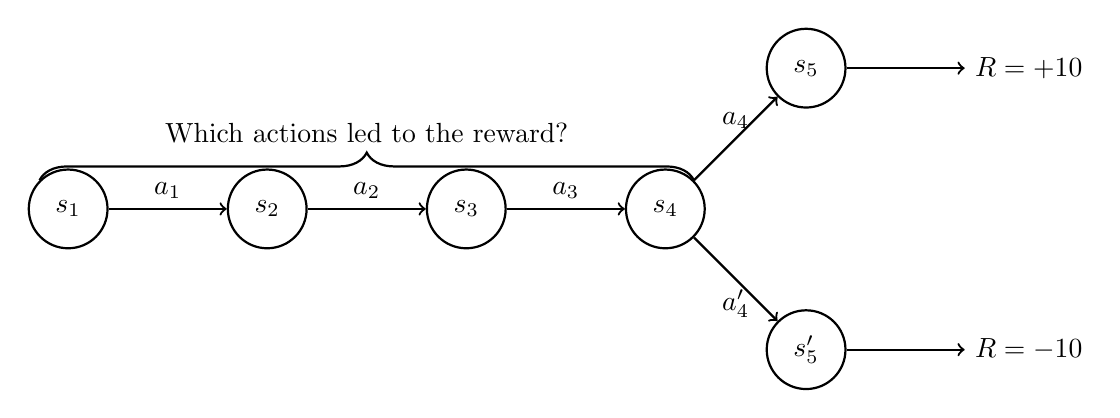
\begin{tikzpicture}[node distance=1.5cm, auto, thick]
    % States
    \node[draw,circle,minimum size=1cm] (s1) {$s_1$};
    \node[draw,circle,minimum size=1cm, right=of s1] (s2) {$s_2$};
    \node[draw,circle,minimum size=1cm, right=of s2] (s3) {$s_3$};
    \node[draw,circle,minimum size=1cm, right=of s3] (s4) {$s_4$};
    \node[draw,circle,minimum size=1cm, above right=of s4] (s5a) {$s_5$};
    \node[draw,circle,minimum size=1cm, below right=of s4] (s5b) {$s_5'$};
    
    % Transitions
    \draw[->] (s1) -- node {$a_1$} (s2);
    \draw[->] (s2) -- node {$a_2$} (s3);
    \draw[->] (s3) -- node {$a_3$} (s4);
    \draw[->] (s4) -- node[above] {$a_4$} (s5a);
    \draw[->] (s4) -- node[below] {$a_4'$} (s5b);
    
    % Rewards
    \node[right=of s5a] (r1) {$R=+10$};
    \node[right=of s5b] (r2) {$R=-10$};
    
    \draw[->] (s5a) -- (r1);
    \draw[->] (s5b) -- (r2);
    
    % Highlight the credit assignment problem
    \draw[decorate,decoration={brace,amplitude=10pt},thick] (s1.north west) -- (s4.north east) node[midway,above=10pt] {Which actions led to the reward?};
\end{tikzpicture}
\caption{The credit assignment problem: determining which actions in a sequence contributed to the final reward}
\end{figure}

In the diagram, a positive reward is received after reaching state $s_5$, and a negative reward after reaching state $s_5'$. The challenge is to determine which of the earlier actions in the sequence (a₁, a₂, a₃, a₄/a₄') were most responsible for the final outcome.

This problem becomes particularly difficult when:
\begin{itemize}
    \item Rewards are delayed (occur many steps after the critical actions)
    \item Actions have long-term consequences through complex state transitions
    \item The environment is noisy or stochastic
\end{itemize}

Reinforcement learning algorithms address this problem through various methods:
\begin{itemize}
    \item \textbf{Temporal Difference Learning}: Updates value estimates based on the difference between successive predictions
    \item \textbf{Eligibility Traces}: Maintain a record of which states and actions have been visited recently and are thus "eligible" for updates
    \item \textbf{Monte Carlo Methods}: Use complete episode returns to update action values
\end{itemize}

\subsection{Comparison: Bandits vs. Contextual Bandits vs. Full RL}

\begin{table}[H]
\centering
\begin{tabular}{|l|c|c|c|}
\hline
\textbf{Feature} & \textbf{Bandits} & \textbf{Contextual Bandits} & \textbf{Full RL} \\
\hline
States & No & Yes & Yes \\
\hline
Reward depends on state & No & Yes & Yes \\
\hline
Actions affect future states & No & No & Yes \\
\hline
Time horizon & Immediate & Immediate & Multiple steps \\
\hline
Value function & $Q(a)$ & $Q(s,a)$ & $q_{\pi}(s,a), v_{\pi}(s)$ \\
\hline
Considers future rewards & No & No & Yes \\
\hline
Credit assignment & Simple & Simple & Complex \\
\hline
Optimal policy computation & Easy & Moderate & Hard \\
\hline
Exploration-exploitation & Simple & Moderate & Complex \\
\hline
\end{tabular}
\caption{Comparison of key features across bandit problems, contextual bandits, and full RL}
\end{table}

\section{Conclusion}

The transition from bandits to full reinforcement learning represents a significant increase in complexity and expressive power:

\begin{itemize}
    \item \textbf{Bandits} involve only actions and immediate rewards with no concept of state.
    \item \textbf{Contextual Bandits} introduce states that influence rewards, but actions don't affect future states.
    \item \textbf{Full RL} incorporates state transitions influenced by actions, creating sequential decision problems where actions have long-term consequences.
\end{itemize}

This progression captures the core challenge of reinforcement learning: making decisions that optimize long-term cumulative reward when actions influence not just immediate rewards but also future states and opportunities.

The key concepts introduced in full reinforcement learning include:
\begin{itemize}
    \item The Markov property, which allows decisions to be based solely on the current state
    \item Value functions, which estimate the expected future reward
    \item The Bellman equations, which express the recursive relationship between values of different states
    \item Optimal policies, which maximize the expected return
    \item The credit assignment problem, which involves determining which actions led to observed rewards
\end{itemize}

Understanding these fundamental concepts provides the foundation for more advanced reinforcement learning methods, including temporal difference learning, Monte Carlo methods, and function approximation techniques.

\section{Summary of Key Equations}

Here is a summary of all the key equations covered in this document:

\subsection{Reward Dependencies}
\begin{align}
&\text{Bandits:} & p(r_t|a_t) \\
&\text{Contextual Bandits:} & p(r_t|s_t, a_t) \\
&\text{Full RL:} & p(r_t|s_t, a_t) \text{ and } p(s_{t+1}|s_t, a_t)
\end{align}

\subsection{MDP Dynamics}
\begin{align}
&\text{Joint Probability:} & p(s',r|s,a) = P(S_t = s', R_t = r|S_{t-1} = s, A_{t-1} = a) \\
&\text{State Transition:} & p(s'|s,a) = \sum_{r \in \mathcal{R}} p(s',r|s,a) \\
&\text{Expected Reward:} & r(s,a) = \sum_{r \in \mathcal{R}} r \sum_{s' \in \mathcal{S}} p(s',r|s,a) \\
&\text{Expected Reward with Next State:} & r(s,a,s') = \sum_{r \in \mathcal{R}} r \frac{p(s',r|s,a)}{p(s'|s,a)}
\end{align}

\subsection{Return}
\begin{align}
&\text{Continuing Tasks:} & G_t = \sum_{k=0}^{\infty} \gamma^k R_{t+k+1} \\
&\text{Episodic Tasks:} & G_t = \sum_{k=0}^{T-t-1} \gamma^k R_{t+k+1} \\
&\text{Unified Notation:} & G_t = \sum_{k=t+1}^{T} \gamma^{k-t-1} R_k
\end{align}

\subsection{Value Functions}
\begin{align}
&\text{State-Value Function:} & v_{\pi}(s) = \mathbb{E}_{\pi}[G_t|S_t = s] \\
&\text{Action-Value Function:} & q_{\pi}(s,a) = \mathbb{E}_{\pi}[G_t|S_t = s, A_t = a] \\
&\text{Relationship:} & v_{\pi}(s) = \sum_{a} \pi(a|s) q_{\pi}(s, a) \\
&\text{Inverse Relationship:} & q_{\pi}(s, a) = \sum_{s', r} p(s', r|s, a) [r + \gamma v_{\pi}(s')]
\end{align}

\subsection{Bellman Equations}
\begin{align}
&\text{For State-Value:} & v_{\pi}(s) = \sum_{a} \pi(a|s) \sum_{s',r} p(s',r|s,a) [r + \gamma v_{\pi}(s')] \\
&\text{For Action-Value:} & q_{\pi}(s,a) = \sum_{s',r} p(s',r|s,a) \left[r + \gamma \sum_{a'} \pi(a'|s') q_{\pi}(s',a') \right]
\end{align}

\subsection{Optimal Value Functions}
\begin{align}
&\text{Optimal State-Value:} & v_*(s) = \max_{\pi} v_{\pi}(s) \\
&\text{Optimal Action-Value:} & q_*(s,a) = \max_{\pi} q_{\pi}(s,a)
\end{align}

\subsection{Bellman Optimality Equations}
\begin{align}
&\text{For State-Value:} & v_*(s) = \max_a \sum_{s',r} p(s',r|s,a) [r + \gamma v_*(s')] \\
&\text{For Action-Value:} & q_*(s,a) = \sum_{s',r} p(s',r|s,a) [r + \gamma \max_{a'} q_*(s',a')]
\end{align}

\subsection{Policies}
\begin{align}
&\text{Policy Definition:} & \pi(a|s) = P(A_t = a | S_t = s) \\
&\text{Greedy Policy:} & \pi(a|s) = 
\begin{cases}
1 & \text{if } a = \arg\max_{a'} Q(s,a') \\
0 & \text{otherwise}
\end{cases} \\
&\text{$\epsilon$-Greedy Policy:} & \pi(a|s) = 
\begin{cases}
1 - \epsilon + \frac{\epsilon}{|\mathcal{A}(s)|} & \text{if } a = \arg\max_{a'} Q(s,a') \\
\frac{\epsilon}{|\mathcal{A}(s)|} & \text{otherwise}
\end{cases} \\
&\text{Softmax Policy:} & \pi(a|s) = \frac{e^{Q(s,a)/\tau}}{\sum_{a'} e^{Q(s,a')/\tau}} \\
&\text{Optimal Policy:} & \pi_*(s) = \arg\max_a q_*(s,a)
\end{align}

\subsection{Estimating Action Values}
\begin{align}
&\text{Averaging Approach:} & Q_t(s,a) = \frac{1}{n_t(s,a)} \sum_{i=1}^{t} r_i \cdot \mathbb{I}(s_i = s, a_i = a) \\
&\text{Incremental Update:} & Q_{t+1}(s_t,a_t) = Q_t(s_t,a_t) + \alpha [r_{t+1} - Q_t(s_t,a_t)]
\end{align}

\end{document}